\PassOptionsToPackage{unicode=true}{hyperref} % options for packages loaded elsewhere
\PassOptionsToPackage{hyphens}{url}
%
\documentclass[]{article}
\usepackage{lmodern}
\usepackage{amssymb,amsmath}
\usepackage{ifxetex,ifluatex}
\usepackage{fixltx2e} % provides \textsubscript
\ifnum 0\ifxetex 1\fi\ifluatex 1\fi=0 % if pdftex
  \usepackage[T1]{fontenc}
  \usepackage[utf8]{inputenc}
  \usepackage{textcomp} % provides euro and other symbols
\else % if luatex or xelatex
  \usepackage{unicode-math}
  \defaultfontfeatures{Ligatures=TeX,Scale=MatchLowercase}
\fi
% use upquote if available, for straight quotes in verbatim environments
\IfFileExists{upquote.sty}{\usepackage{upquote}}{}
% use microtype if available
\IfFileExists{microtype.sty}{%
\usepackage[]{microtype}
\UseMicrotypeSet[protrusion]{basicmath} % disable protrusion for tt fonts
}{}
\IfFileExists{parskip.sty}{%
\usepackage{parskip}
}{% else
\setlength{\parindent}{0pt}
\setlength{\parskip}{6pt plus 2pt minus 1pt}
}
\usepackage{hyperref}
\hypersetup{
            pdfborder={0 0 0},
            breaklinks=true}
\urlstyle{same}  % don't use monospace font for urls
\usepackage{color}
\usepackage{fancyvrb}
\newcommand{\VerbBar}{|}
\newcommand{\VERB}{\Verb[commandchars=\\\{\}]}
\DefineVerbatimEnvironment{Highlighting}{Verbatim}{commandchars=\\\{\}}
% Add ',fontsize=\small' for more characters per line
\newenvironment{Shaded}{}{}
\newcommand{\AlertTok}[1]{\textcolor[rgb]{1.00,0.00,0.00}{\textbf{#1}}}
\newcommand{\AnnotationTok}[1]{\textcolor[rgb]{0.38,0.63,0.69}{\textbf{\textit{#1}}}}
\newcommand{\AttributeTok}[1]{\textcolor[rgb]{0.49,0.56,0.16}{#1}}
\newcommand{\BaseNTok}[1]{\textcolor[rgb]{0.25,0.63,0.44}{#1}}
\newcommand{\BuiltInTok}[1]{#1}
\newcommand{\CharTok}[1]{\textcolor[rgb]{0.25,0.44,0.63}{#1}}
\newcommand{\CommentTok}[1]{\textcolor[rgb]{0.38,0.63,0.69}{\textit{#1}}}
\newcommand{\CommentVarTok}[1]{\textcolor[rgb]{0.38,0.63,0.69}{\textbf{\textit{#1}}}}
\newcommand{\ConstantTok}[1]{\textcolor[rgb]{0.53,0.00,0.00}{#1}}
\newcommand{\ControlFlowTok}[1]{\textcolor[rgb]{0.00,0.44,0.13}{\textbf{#1}}}
\newcommand{\DataTypeTok}[1]{\textcolor[rgb]{0.56,0.13,0.00}{#1}}
\newcommand{\DecValTok}[1]{\textcolor[rgb]{0.25,0.63,0.44}{#1}}
\newcommand{\DocumentationTok}[1]{\textcolor[rgb]{0.73,0.13,0.13}{\textit{#1}}}
\newcommand{\ErrorTok}[1]{\textcolor[rgb]{1.00,0.00,0.00}{\textbf{#1}}}
\newcommand{\ExtensionTok}[1]{#1}
\newcommand{\FloatTok}[1]{\textcolor[rgb]{0.25,0.63,0.44}{#1}}
\newcommand{\FunctionTok}[1]{\textcolor[rgb]{0.02,0.16,0.49}{#1}}
\newcommand{\ImportTok}[1]{#1}
\newcommand{\InformationTok}[1]{\textcolor[rgb]{0.38,0.63,0.69}{\textbf{\textit{#1}}}}
\newcommand{\KeywordTok}[1]{\textcolor[rgb]{0.00,0.44,0.13}{\textbf{#1}}}
\newcommand{\NormalTok}[1]{#1}
\newcommand{\OperatorTok}[1]{\textcolor[rgb]{0.40,0.40,0.40}{#1}}
\newcommand{\OtherTok}[1]{\textcolor[rgb]{0.00,0.44,0.13}{#1}}
\newcommand{\PreprocessorTok}[1]{\textcolor[rgb]{0.74,0.48,0.00}{#1}}
\newcommand{\RegionMarkerTok}[1]{#1}
\newcommand{\SpecialCharTok}[1]{\textcolor[rgb]{0.25,0.44,0.63}{#1}}
\newcommand{\SpecialStringTok}[1]{\textcolor[rgb]{0.73,0.40,0.53}{#1}}
\newcommand{\StringTok}[1]{\textcolor[rgb]{0.25,0.44,0.63}{#1}}
\newcommand{\VariableTok}[1]{\textcolor[rgb]{0.10,0.09,0.49}{#1}}
\newcommand{\VerbatimStringTok}[1]{\textcolor[rgb]{0.25,0.44,0.63}{#1}}
\newcommand{\WarningTok}[1]{\textcolor[rgb]{0.38,0.63,0.69}{\textbf{\textit{#1}}}}
\usepackage{longtable,booktabs}
% Fix footnotes in tables (requires footnote package)
\IfFileExists{footnote.sty}{\usepackage{footnote}\makesavenoteenv{longtable}}{}
\usepackage{graphicx,grffile}
\makeatletter
\def\maxwidth{\ifdim\Gin@nat@width>\linewidth\linewidth\else\Gin@nat@width\fi}
\def\maxheight{\ifdim\Gin@nat@height>\textheight\textheight\else\Gin@nat@height\fi}
\makeatother
% Scale images if necessary, so that they will not overflow the page
% margins by default, and it is still possible to overwrite the defaults
% using explicit options in \includegraphics[width, height, ...]{}
\setkeys{Gin}{width=\maxwidth,height=\maxheight,keepaspectratio}
\setlength{\emergencystretch}{3em}  % prevent overfull lines
\providecommand{\tightlist}{%
  \setlength{\itemsep}{0pt}\setlength{\parskip}{0pt}}
\setcounter{secnumdepth}{0}
% Redefines (sub)paragraphs to behave more like sections
\ifx\paragraph\undefined\else
\let\oldparagraph\paragraph
\renewcommand{\paragraph}[1]{\oldparagraph{#1}\mbox{}}
\fi
\ifx\subparagraph\undefined\else
\let\oldsubparagraph\subparagraph
\renewcommand{\subparagraph}[1]{\oldsubparagraph{#1}\mbox{}}
\fi

% set default figure placement to htbp
\makeatletter
\def\fps@figure{htbp}
\makeatother


\date{}

\begin{document}

\hypertarget{header-n2}{%
\section{\texorpdfstring{\(\ell_1\) Image
Inpainting}{\textbackslash{}ell\_1 Image Inpainting}}\label{header-n2}}

The \(\ell_1\)-regularized image reconstruction is an alternative method
to solve the image inpainting problem:
\begin{equation}
{x\in\R^{mn}}\  ||\Psi x||_1\qquad\text{s.t.}\qquad ||Ax-b||_\infty\le\delta,\tag3
\end{equation}
where \(\Psi_{mn\times mn}\) transfers the image \(x\) to the frequency
domain; \(A_{s\times mn}\) and \(b\in\R^s\) are as in the Total
Variation Minimization Problem formulation, and \(\delta\gt\mathbb0\) is
the error threshold between the undamaged pixels \(b\) and the
reconstructed version \(Ax.\)

We derived the linear programming formulation of \((3)\) as well as its
dual problem. We implemented and tested the the program on sample
grey-scale images. We examined the reconstruction quality and speed of
the model under different sets of parameters.

\hypertarget{header-n7}{%
\subsection{LP formulation}\label{header-n7}}

We first reformulate \((3)\) as a linear program by noting that

\begin{aligned}

&\quad\ \min_{x\in\R^{mn}}\  ||\Psi x||_1\qquad\text{s.t.}\qquad ||Ax-b||_\infty\le\delta\\



&=\min_{x\in\R^{mn}}\  \mathbf1^\top |\Psi x|\qquad\text{s.t.}\qquad \left|A x-b\right|\le\delta\mathbf1\\



&=\min_{x,t\in\R^{mn}}\  \mathbf1^\top t\qquad\text{s.t.}\qquad t\ge\pm\Psi x, \quad \pm\left(A x-b\right)\le\delta\mathbf1.



\end{aligned}\tag4

Here, \(\mathbf1\) denotes the all-one vectors of appropriate sizes and
\(|v|\) is interpreted element-wise on vector \(v.\)

\hypertarget{header-n12}{%
\subsection{Dual problem}\label{header-n12}}

Next, we derive the associated dual of \((4).\) Rewrite \((4)\)

\begin{aligned}
&\quad\ \min_{x,t\in\R^{mn}}\  \mathbf1^\top t\qquad\text{s.t.}\qquad t\ge\pm\Psi x, \quad \pm\left(A x-b\right)\le\delta\mathbf1
\\&=\min_{x,t\in\R^{mn}}\mathbf1^\top t\qquad\text{s.t.}\qquad 
\pm\Psi x+t\ge0,\quad\pm A x\ge-\delta\mathbf1\pm b\\
&=\min_{x,t\in\R^{mn}} \left[0^\top|\ \mathbf1^\top\right]\left[\begin{array}{c}
x\\t
\end{array}\right]\qquad\text{s.t.}\qquad
\left[\begin{array}{cc}
\Psi&I_{mn}\\
-\Psi&I_{mn}\\
A& 0_{s\times mn}\\
-A&0_{s\times mn}
\end{array}\right]
\left[\begin{array}{c}
x\\t
\end{array}\right]\ge
\left[\begin{array}{c}
0\\0\\-\delta\mathbf1+ b
\\-\delta\mathbf1- b
\end{array}\right].
\end{aligned}

where \(I_r\) denotes the \(r\times r\) identity matrix and
\(0_{p\times q}\) is the \(p\times q\) all-zero matrix.

The dual is then given by

\begin{aligned}

&\quad\ \max_{u,v\in\R^{mn}\\y,z\in\R^{s}} \left[0^\top|\ 0^\top|-\delta\mathbf1^\top+ b^\top\ |-\delta\mathbf1^\top- b^\top\right]\left[\begin{array}{c}

u & v & y & z

\end{array}\right]^\top

\\

&\qquad\ \text{s.t.}\qquad

\left[\begin{array}{cc}

\Psi^\top&-\Psi^\top&A^\top&-A^\top\\

I_{mn}&I_{mn}&0_{mn\times s}&0_{mn\times s}\\

\end{array}\right]

\left[\begin{array}{c}

u&v&y&z

\end{array}\right]^\top

=

\left[\begin{array}{c}

0\\\mathbf1

\end{array}\right],\quad u,v,y,z\ge0\\\\&=

\max_{u,v\in\R^{mn}\\y,z\in\R^{s}}\ b^\top(y-z)-\delta\mathbf1^\top(y+z)\\

&\qquad\text{s.t.}\qquad \Psi^\top(u-v)+A^\top(y-z)=0,\quad u+v= \mathbf1,\quad u,v,y,z\ge0\\\\&=

\max_{t\in\R^{mn}\\r,w\in\R^{s}}\ b^\top w-\delta\mathbf1^\top(w+r)\\

&\qquad\ \text{s.t.}\qquad \Psi^\top t+A^\top w=0,\quad r\ge0,\quad -1\le t\le1\\\\&=

\max_{t\in\R^{mn}\\w\in\R^{s}}\ \left(b^\top -\delta\mathbf1^\top\right) w\\

&\qquad\text{s.t.}\qquad \Psi^\top t+A^\top w=0,\quad -1\le t\le1.

\end{aligned}

\hypertarget{header-n19}{%
\subsection{Implementation}\label{header-n19}}

We implemented the \(\ell_1\) inpainting algorithm with \texttt{linprog}
function in MATLAB R2020a. The \texttt{interior-point} method was chosen
for speed concern.

\begin{Shaded}
\begin{Highlighting}[]
\CommentTok{% parameters, preprocesses of image and mask
}
\NormalTok{U       = imread(}\StringTok{'.\textbackslash{}test_images\textbackslash{}512_512_lena.png'}\NormalTok{);
}
\NormalTok{if size(U, }\FloatTok{3}\NormalTok{) == }\FloatTok{3}

\NormalTok{    U 	= rgb2gray(U);
}
\NormalTok{end
}
\NormalTok{U       = double(U) / }\FloatTok{255}\NormalTok{;
}
\NormalTok{[m, n]  = size(U);
}


\NormalTok{Ind     = imread(}\StringTok{'.\textbackslash{}test_masks\textbackslash{}512_512_random50.png'}\NormalTok{);
}
\NormalTok{Ind     = logical(ceil(Ind / }\FloatTok{255}\NormalTok{));
}
\NormalTok{s       = sum(Ind, }\StringTok{'all'}\NormalTok{);
}
\NormalTok{delta   = }\FloatTok{0.06}\NormalTok{;
}


\NormalTok{bsz = }\FloatTok{8}\NormalTok{;
}
\NormalTok{Psi = get_Psi(m, n, bsz);
}


\CommentTok{% block-stack U and Ind in Psi style
}
\NormalTok{u   = blk_stack(U, bsz);
}
\NormalTok{ind = blk_stack(Ind, bsz);
}


\CommentTok{% form A and b
}
\NormalTok{i       = }\FloatTok{1}\NormalTok{:s;
}
\NormalTok{j       = zeros(}\FloatTok{1}\NormalTok{,s);
}
\NormalTok{count   = }\FloatTok{1}\NormalTok{;
}
\NormalTok{for col = }\FloatTok{1}\NormalTok{:m*n
}
\NormalTok{    if ind(col) == }\FloatTok{1}

\NormalTok{        j(count) = col;
}
\NormalTok{        count = count + }\FloatTok{1}\NormalTok{;
}
\NormalTok{    end
}
\NormalTok{end
}
\NormalTok{A = sparse(i, j, ones(}\FloatTok{1}\NormalTok{, s), s, m*n);
}
\NormalTok{b = A * u;
}


\CommentTok{% linprog
}
\CommentTok{% min(c'x) s.t. Mx <= d
}
\NormalTok{del     = delta*ones(s, }\FloatTok{1}\NormalTok{);
}
\NormalTok{I       = speye(m*n);
}
\NormalTok{ze      = sparse(s, m*n);
}
\NormalTok{c       = [zeros(m*n, }\FloatTok{1}\NormalTok{); ones(m*n, }\FloatTok{1}\NormalTok{)];
}
\NormalTok{M       = [-Psi -I; Psi -I; -A ze; A ze];
}
\NormalTok{d       = [zeros(}\FloatTok{2}\NormalTok{*m*n, }\FloatTok{1}\NormalTok{); del-b; del+b];
}
\NormalTok{options = optimoptions(}\StringTok{'linprog'}\NormalTok{, }\StringTok{'Algorithm'}\NormalTok{, }\StringTok{'interior-point'}\NormalTok{, ...
}
                       \StringTok{'ConstraintTolerance'}\NormalTok{, }\FloatTok{1e-3}\NormalTok{, }\StringTok{'Display'}\NormalTok{, }\StringTok{'iter'}\NormalTok{);
}
\NormalTok{x       = linprog(c, M, d, [], [], [], [], options);
}


\CommentTok{% scale and transform the stacked image back into matrix
}
\NormalTok{x = uint8( x(}\FloatTok{1}\NormalTok{:m*n)*}\FloatTok{255}\NormalTok{ );
}
\NormalTok{X = blk_unstack(x, bsz);
}


\CommentTok{% evaluate PSNR
}
\NormalTok{psnr = PSNR((U*}\FloatTok{255}\NormalTok{), double(X));
}
\NormalTok{imshow(X);}
\end{Highlighting}
\end{Shaded}

\hypertarget{header-n23}{%
\subsection{Results}\label{header-n23}}

We tested the model on sample grey-scale images of \(256\times256\) and
\(512\times512\) pixels. The results were obtained with a 4.0 GHz
Quad-Core Intel Core i7-4790K processor and 32 GB 2133 MHz memory. The
quality of the reconstructed images was assessed via the PSNR value:

\[\text{PSNR}:=10\cdot\log_{10}\frac{mn}{||x-u^*||^2},\]

where \(x\) is the reconstructed image and \(u^*=\text{vec}(U^*)\) is
the ground truth.

\hypertarget{header-n28}{%
\subsubsection{Overall performance}\label{header-n28}}

The \(\ell_1\) block model reconstructs \(256\times256\) images
contaminated by \(50\%\) random noise with \(\text{PSNR}\approx 20.\)
The average runtime is around \(40\text{ sec}\) with a maximum of \(20\)
iterations. We notice that the algorithm takes significantly longer at
each iteration, and more iterations to converge, if the block size
\(\text{bsz}\) is set at \(16\) (the value recommended by the lecturer
for low-res images). For instance, image \((\mathbf a)\) takes nearly
\(8\text{ min}\) to reconstruct at \(\text{bsz}=16,\) along with a
\(2.3\) increase in PSNR, and images \((\mathbf b)\) and \((\mathbf c)\)
fail to converge within a \(200\)-iteration limit. After examining
matrix \(\Psi,\) we find that it is because the number of non-zero
elements \(\Psi\) increase proportionally to \(\text{bsz}^2,\) resulting
in significantly more computations.

\begin{longtable}[]{@{}llllll@{}}
\toprule
& Ground Truth & Ground Truth + \(50\%\) Noise & Reconstructed Images &
PSNR & Runtime (Iterations)\tabularnewline
\midrule
\endhead
\((\mathbf a)\) &
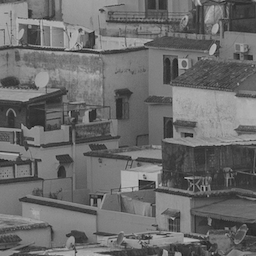
\includegraphics{C:/Users/Jamie/Documents/University-Stuffs/MAT3007/Midterm/c.PNG}
&
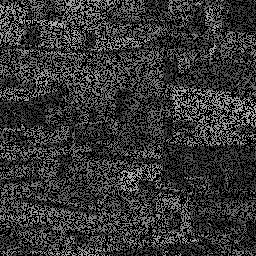
\includegraphics{C:/Users/Jamie/Documents/University-Stuffs/MAT3007/Midterm/test_results/masked/2 (2).png}
&
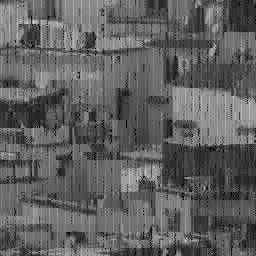
\includegraphics{C:/Users/Jamie/Documents/University-Stuffs/MAT3007/Midterm/buildings_bsz_8_21.6.png}
& \(21.6\) & \(38.4\text{ sec}\\(17)\)\tabularnewline
\((\text{bsz}=16)\) & & &
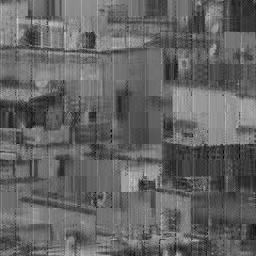
\includegraphics{C:/Users/Jamie/Documents/University-Stuffs/MAT3007/Midterm/test_results/256/256_house+rand_50_del0.06_474s.png}
& \(23.9\) & \(7.9\text{ min}\)\tabularnewline
\((\mathbf b)\) &
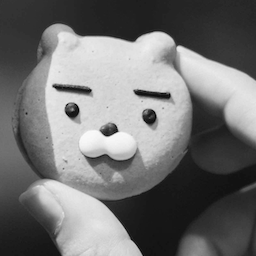
\includegraphics{C:/Users/Jamie/Documents/University-Stuffs/MAT3007/Midterm/B.PNG}
&
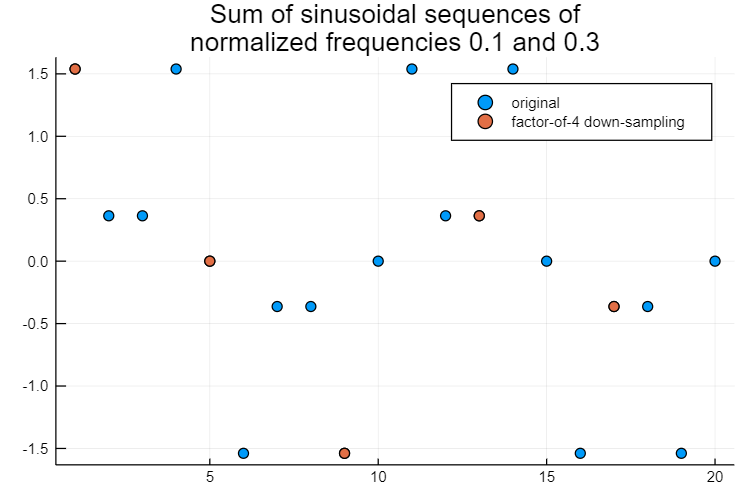
\includegraphics{C:/Users/Jamie/Documents/University-Stuffs/MAT3007/Midterm/test_results/masked/2.png}
&
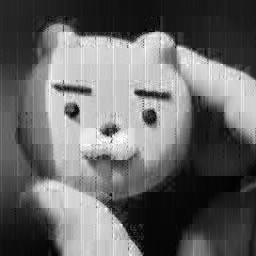
\includegraphics{C:/Users/Jamie/Documents/University-Stuffs/MAT3007/Midterm/test_results/256/256_hand+random_50_del0.06_s.png}
& \(22.3\) & \(44.2\text{    sec}\\(20)\)\tabularnewline
\((\mathbf c)\) &
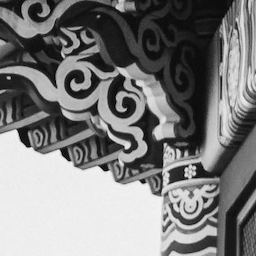
\includegraphics{C:/Users/Jamie/Documents/University-Stuffs/MAT3007/Midterm/A.PNG}
&
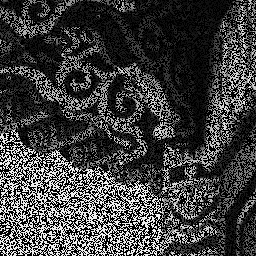
\includegraphics{C:/Users/Jamie/Documents/University-Stuffs/MAT3007/Midterm/test_results/masked/casino.png}
&

\includegraphics{C:/Users/Jamie/Documents/University-Stuffs/MAT3007/Midterm/test_results/256/256_casino+rand_50_del0.06_49s.png}
& \(20.4\) & \(44.5\text{    sec}\\ (19)\)\tabularnewline
\bottomrule
\end{longtable}

\emph{Table 1.} \(\ell_1\) inpainting results of \(256\times256\) images
contaminated by \(50\%\) random noise, \(\delta=6\times10^{-2},\)
\(\text{bsz}=8,\) constraint tolerance \(= 10^{-3},\) optimality
tolerance \(= 10^{-6}\)

\begin{figure}
\centering
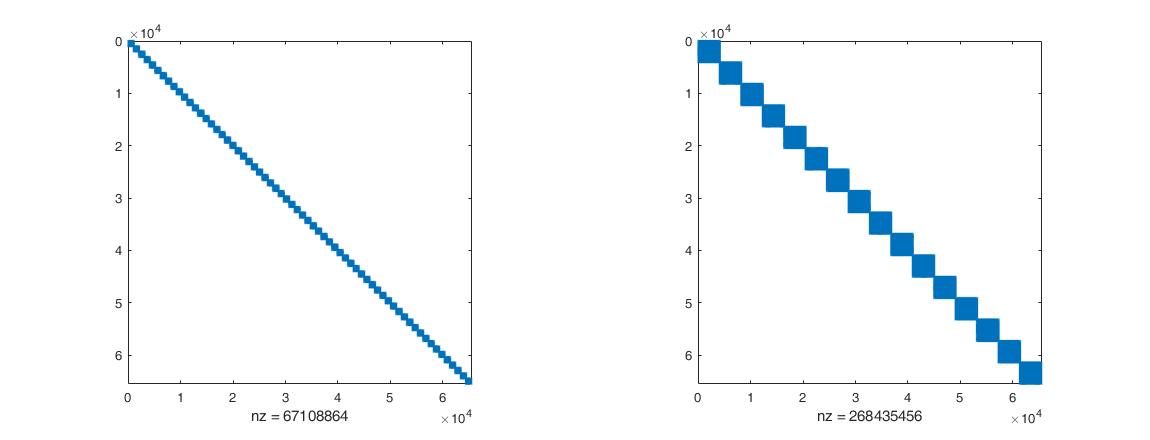
\includegraphics{C:/Users/Jamie/Documents/University-Stuffs/MAT3007/Midterm/test_results/Psi/bsz.png}
\caption{bsz}
\end{figure}

\emph{Figure 1.} Sparsity patterns of \(\Psi\) with \(\text{bsz}=32\)
(Left) and \(\text{bsz}=64\) (Right), \(m=n=256\)

In the task of reconstructing \(512\times512\) image polluted by
\(50\%\) random noise, the algorithm achieves roughly the same
\(\text{PSNR}\) compared to low-res images within similar number of
iterations, while the runtime becomes roughly four times as long. We
also observed that as the noise intensity increased, the image quality
deteriorates drastically although the algorithm seems to converge
faster.

\begin{longtable}[]{@{}lllll@{}}
\toprule
Noise Percentage & Ground Truth & \(30\%\) & \(50\%\) &
\(70\%\)\tabularnewline
\midrule
\endhead
\textbf{Ground Truth + Noise} &
\textbf{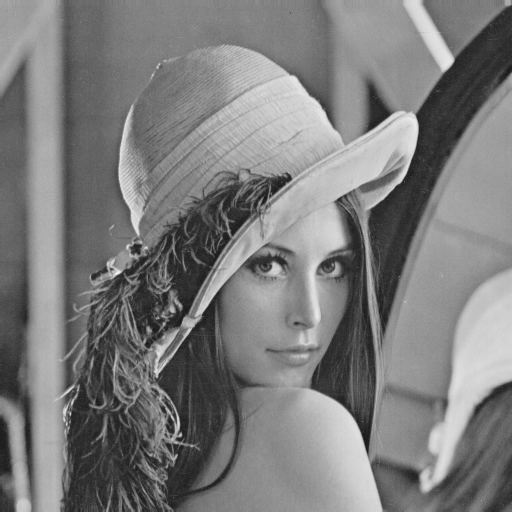
\includegraphics{C:/Users/Jamie/Documents/University-Stuffs/MAT3007/Midterm/test_images/512_512_lena.png}}
&
\textbf{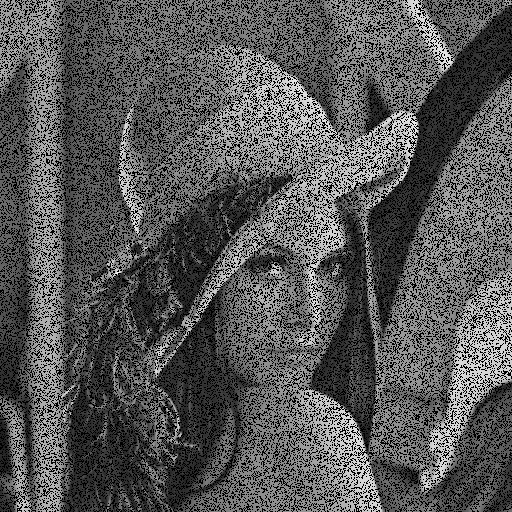
\includegraphics{C:/Users/Jamie/Documents/University-Stuffs/MAT3007/Midterm/test_results/masked/lena_rand30.png}}
&
\textbf{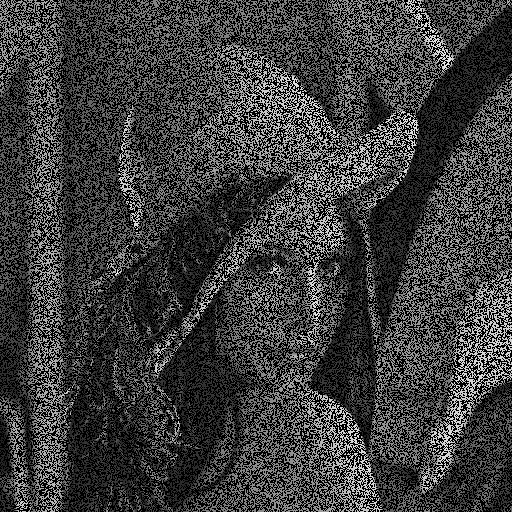
\includegraphics{C:/Users/Jamie/Documents/University-Stuffs/MAT3007/Midterm/test_results/masked/lena_rand50.png}}
&
\textbf{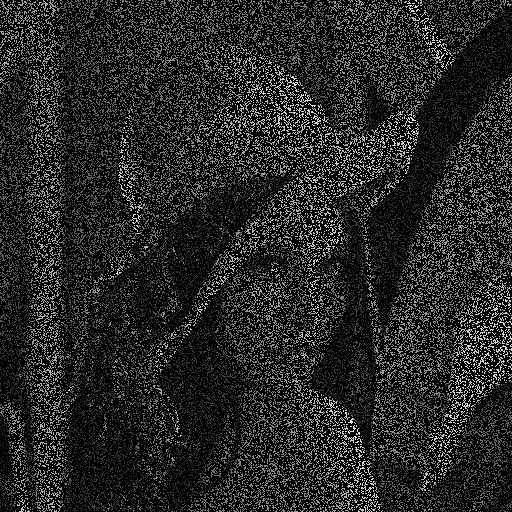
\includegraphics{C:/Users/Jamie/Documents/University-Stuffs/MAT3007/Midterm/test_results/masked/lena_rand70.png}}\tabularnewline
\textbf{Reconstructed Images} & \textbf{-} &
\textbf{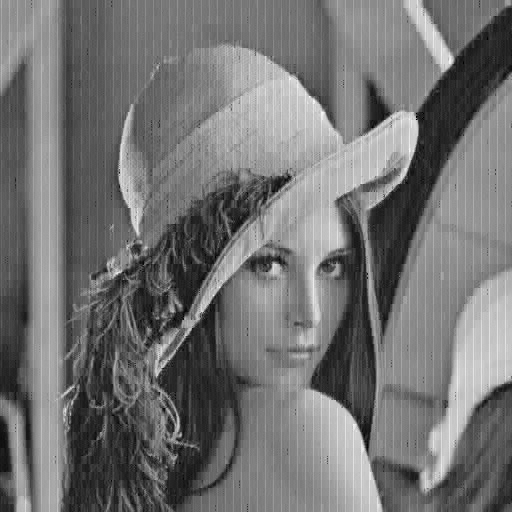
\includegraphics{C:/Users/Jamie/Documents/University-Stuffs/MAT3007/Midterm/test_results/noise_cmp/512_lena+rand_30_del0.06_265s_25.5.png}}
&
\textbf{\includegraphics{C:/Users/Jamie/Documents/University-Stuffs/MAT3007/Midterm/test_results/noise_cmp/512_lena+rand_50_del0.06_186s_22.6.png}}
&
\textbf{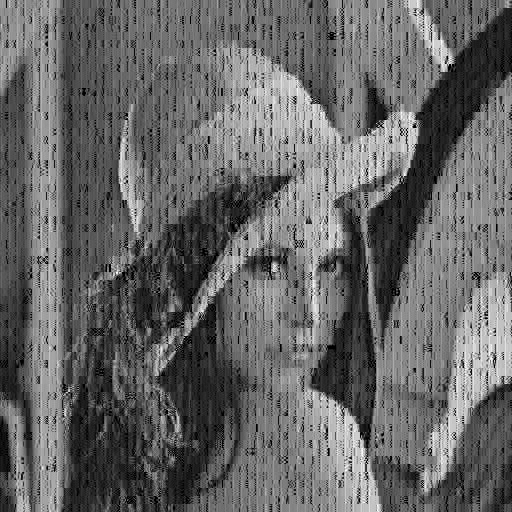
\includegraphics{C:/Users/Jamie/Documents/University-Stuffs/MAT3007/Midterm/test_results/noise_cmp/512_lena+rand_70_del0.06_170s_17.png}}\tabularnewline
\textbf{PSNR} & \textbf{-} & \textbf{\(25.5\)} & \textbf{\(22.6\)} &
\textbf{\(17.0\)}\tabularnewline
\textbf{Runtime (Iterations)} & - & \(4.4\text{ min}\ (26)\) &
\(3.1\text{ min}\ (21)\) & \(2.8\text{ min}\ (21)\)\tabularnewline
\bottomrule
\end{longtable}

\emph{Table 2.} \(\ell_1\) inpainting results of \(512\times512\) images
contaminated by \(30\%,50\%,\) and \(70\%\) random noises,
\(\delta=6\times10^{-2}, \text{bsz}=8,\) constraint tolerance
\(= 10^{-3},\) optimality tolerance \(= 10^{-6}\)

In reconstructing images with non-random damages, the algorithm performs
roughly the same as in the \(50\%\) random noise case with mesh,
handwriting, and mild scratches. However, when inpainting the
hard-scratched image, the algorithm performs poorly with
\(\text{PSNR} = 13.9,\) a score even lower than with the \(70\%\) random
noise, which covers more area of the image than the scratches. From
this, we conclude that the algorithm is sensitive to the distribution of
the damage. In particular, the algorithm performs better if the damage
distributes more evenly, i.e., there is no large "chunks" of damage area
on the image (as in hard scratches).

\begin{longtable}[]{@{}llllll@{}}
\toprule
Damage Types & Ground Truth & Mesh & Handwriting & Mild Scratches & Hard
Scratches\tabularnewline
\midrule
\endhead
\textbf{Damaged Images} &
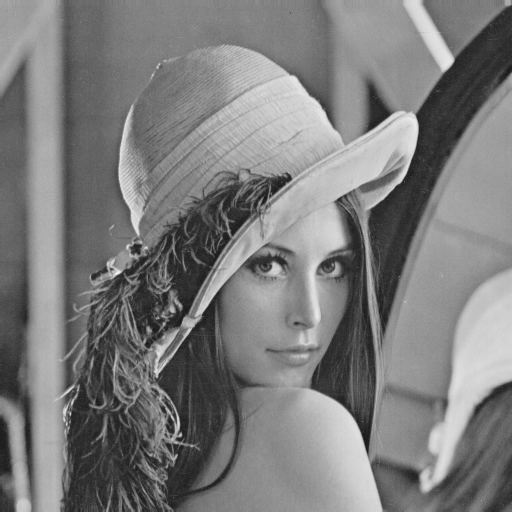
\includegraphics{C:/Users/Jamie/Documents/University-Stuffs/MAT3007/Midterm/test_images/512_512_lena.png}
&
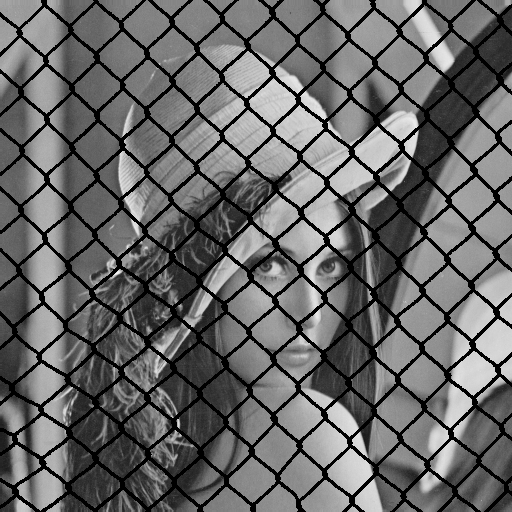
\includegraphics{C:/Users/Jamie/Documents/University-Stuffs/MAT3007/Midterm/mesh.png}
&
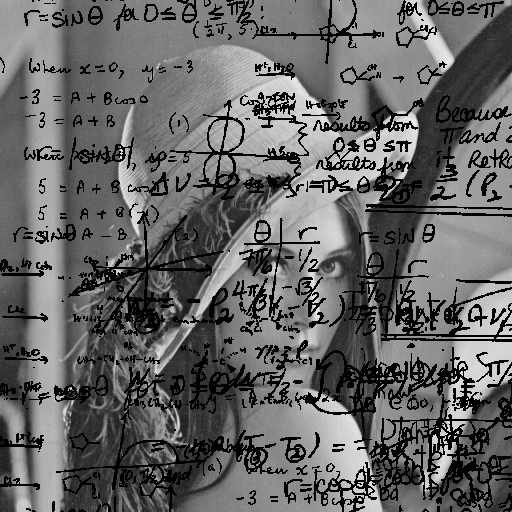
\includegraphics{C:/Users/Jamie/Documents/University-Stuffs/MAT3007/Midterm/handwritting.png}
&
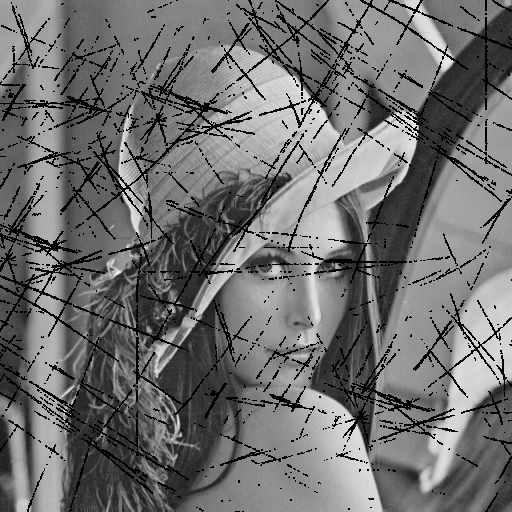
\includegraphics{C:/Users/Jamie/Documents/University-Stuffs/MAT3007/Midterm/scratch1.png}
&
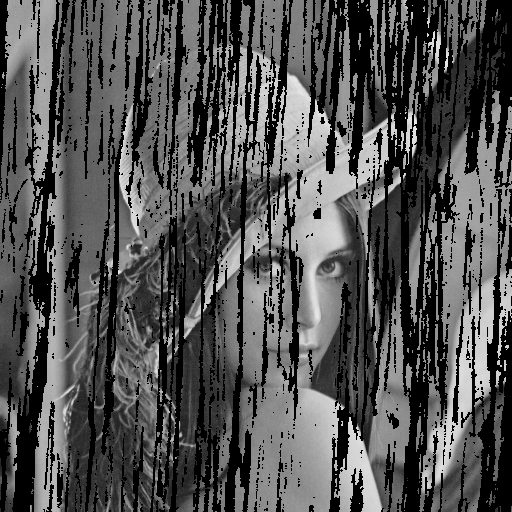
\includegraphics{C:/Users/Jamie/Documents/University-Stuffs/MAT3007/Midterm/scratch.png}\tabularnewline
\textbf{Reconstructed Images} & - &
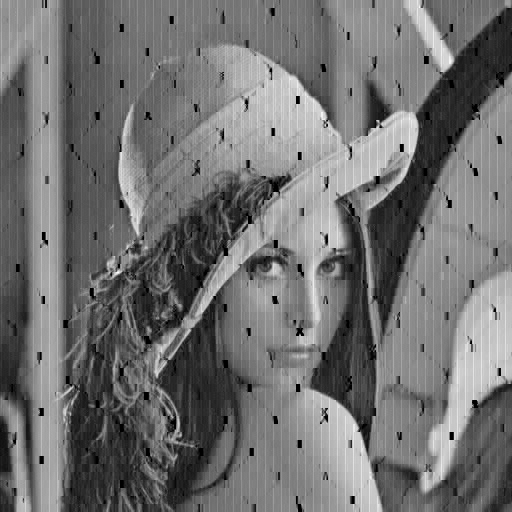
\includegraphics{C:/Users/Jamie/Documents/University-Stuffs/MAT3007/Midterm/test_results/mask_cmp/512_lena+mesh_del0.06_253s_21.6.png}
&
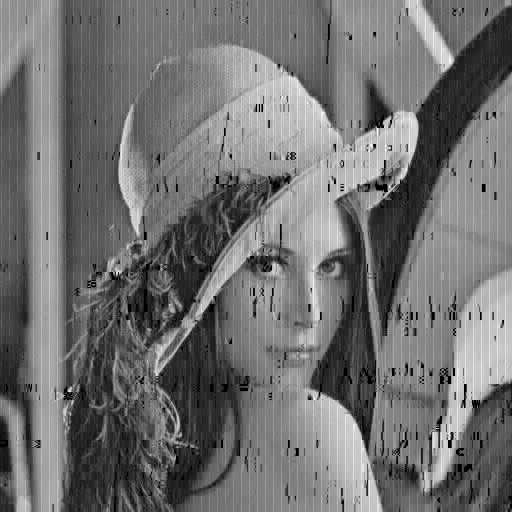
\includegraphics{C:/Users/Jamie/Documents/University-Stuffs/MAT3007/Midterm/test_results/mask_cmp/512_lena+writing_50_del0.06_253s_21.5.png}
&
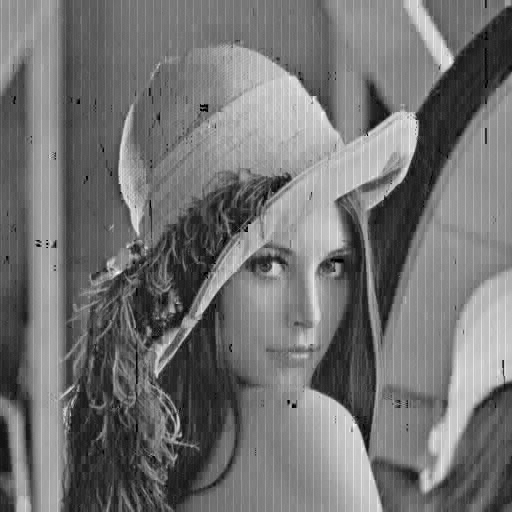
\includegraphics{C:/Users/Jamie/Documents/University-Stuffs/MAT3007/Midterm/scratch1_FIX.png}
&
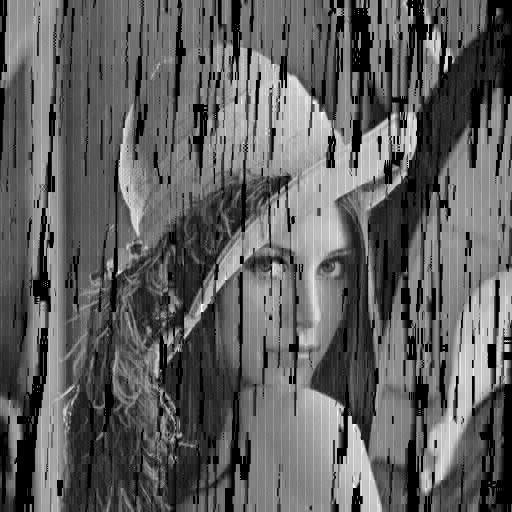
\includegraphics{C:/Users/Jamie/Documents/University-Stuffs/MAT3007/Midterm/scratch_FIX.png}\tabularnewline
\textbf{PSNR} & - & \(21.6 \) & \(21.5\) & \(25.3\) &
\(13.9\)\tabularnewline
\textbf{Runtime (Iterations)} & - & \(4.2\text{ min}\ (26)\) &
\(4.2\text{ min}\ (21)\) & \(4.4\text{ min}\ (24)\) &
\(3.7\text{ min}\ (22)\)\tabularnewline
\bottomrule
\end{longtable}

\emph{Table 3.} \(\ell_1\) inpainting results of \(512\times512\) images
with non-random damage, \(\delta=6\times10^{-2},\) \(\text{bsz}=8,\)
constraint tolerance \(= 10^{-3},\) optimality tolerance \(= 10^{-6}\)

\hypertarget{header-n146}{%
\subsubsection{Effects of adjusting termination
tolerances}\label{header-n146}}

We investigate the effects of adjusting optimality tolerance on the
reconstruction quality by inpainting the \(50\%\) random noise
contaminated image. We observe almost no changes either in image quality
or runtime, when optimality tolerance ranges from \(10^{-7}\) to
\(10^{-5}.\) Curiously, when optimality tolerance is larger than
\(10^{-4},\) the algorithm gets significantly slower and fails to
converge within \(200\) iterations.

\begin{longtable}[]{@{}llllll@{}}
\toprule
Optimality Tolerance & Ground Truth & \(10^{-3,-4}\) & \(10^{-5}\) &
\(10^{-6}\) & \(10^{-7}\)\tabularnewline
\midrule
\endhead
\textbf{Reconstructed Images} &
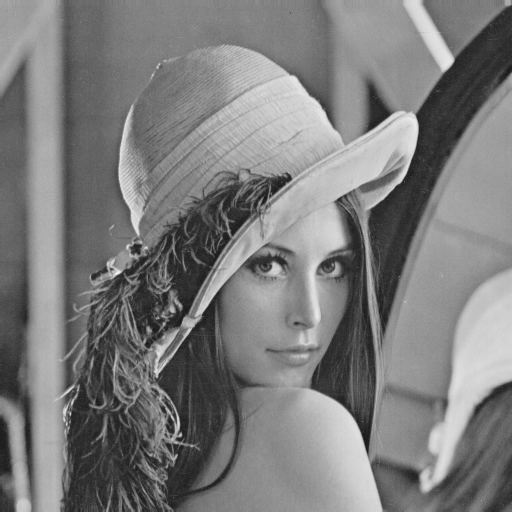
\includegraphics{C:/Users/Jamie/Documents/University-Stuffs/MAT3007/Midterm/test_images/512_512_lena.png}
& - &
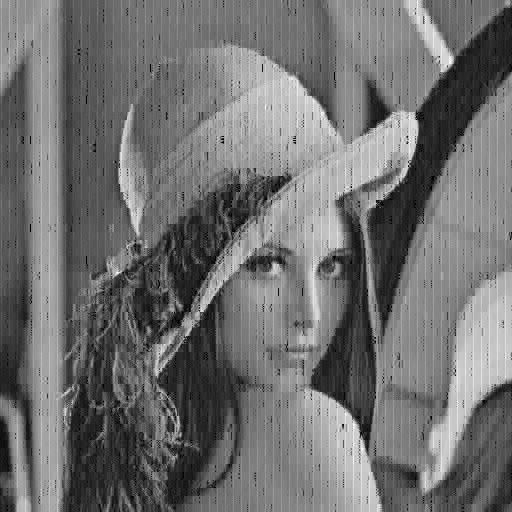
\includegraphics{C:/Users/Jamie/Documents/University-Stuffs/MAT3007/Midterm/test_results/optol_cmp/optol_e-5.png}
&
\includegraphics{C:/Users/Jamie/Documents/University-Stuffs/MAT3007/Midterm/test_results/delta_cmp/512_lena+rand_50_del0.06_186s_22.6.png}
&
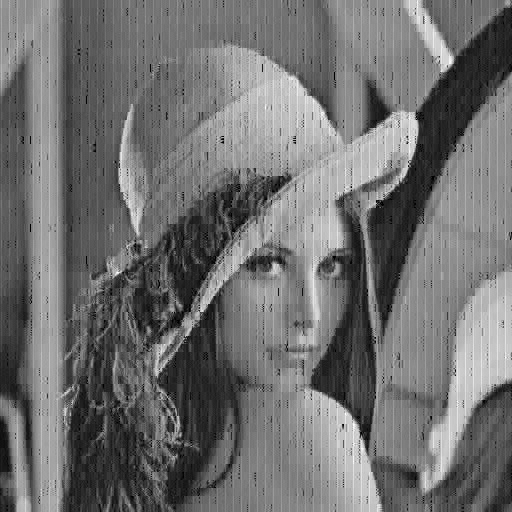
\includegraphics{C:/Users/Jamie/Documents/University-Stuffs/MAT3007/Midterm/test_results/optol_cmp/optol_e-7.png}\tabularnewline
\textbf{PSNR} & - & - & \(22.6\) & \(22.6\) & \(22.6\)\tabularnewline
\textbf{Runtime (Iterations)} & - & \((>200)\) & \(4.4\text{ min }(29)\)
& \(3.1\text{ min}\ (21)\) & \(3.5\text{ min}\ (23)\)\tabularnewline
\bottomrule
\end{longtable}

\emph{Table 4.} Effects of adjusted optimality tolerance on \(\ell_1\)
inpainting results of \(512\times512\) images contaminated by \(50\%\)
random noise, \(\delta=6\times10^{-2}, \text{bsz}=8,\) constraint
tolerance \(= 10^{-3}\)

Our results also suggest the constraint tolerance has no significant
impacts on reconstruction quality or speed. However when constraint
tolerance is below \(10^{-6},\) the algorithm is significantly slower
and struggles to converge within the \(200\)-iteration limit.

\begin{longtable}[]{@{}llllll@{}}
\toprule
Constraint Tolerance & Ground Truth & \(10^{-3}\) & \(10^{-4}\) &
\(10^{-5}\) & \(10^{-6,-7}\)\tabularnewline
\midrule
\endhead
\textbf{Reconstructed Images} &
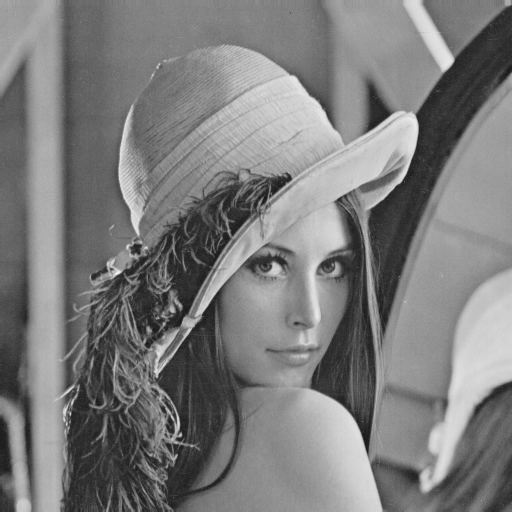
\includegraphics{C:/Users/Jamie/Documents/University-Stuffs/MAT3007/Midterm/test_images/512_512_lena.png}
&
\includegraphics{C:/Users/Jamie/Documents/University-Stuffs/MAT3007/Midterm/test_results/delta_cmp/512_lena+rand_50_del0.06_186s_22.6.png}
&
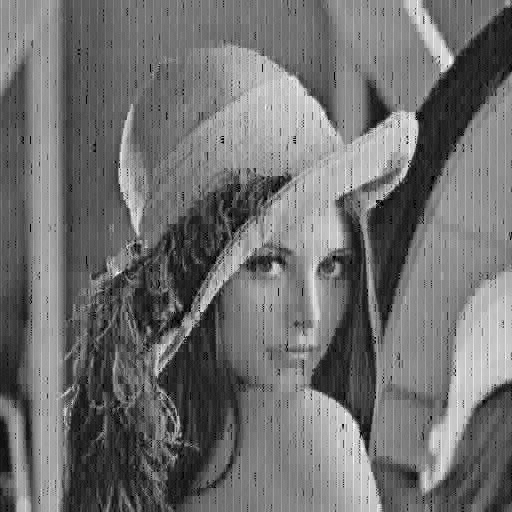
\includegraphics{C:/Users/Jamie/Documents/University-Stuffs/MAT3007/Midterm/test_results/contol_cmp/contol_e-4.png}
&
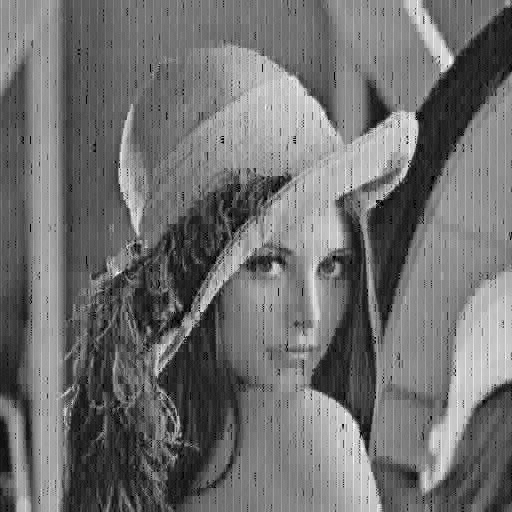
\includegraphics{C:/Users/Jamie/Documents/University-Stuffs/MAT3007/Midterm/test_results/contol_cmp/contol_e-5.png}
& -\tabularnewline
\textbf{PSNR} & - & \(22.6\) & \(22.6\) & \(22.6\) & -\tabularnewline
\textbf{Runtime (Iterations)} & - & \(3.1\text{ min}\ (21)\) &
\(3.5\text{ min}\ (22)\) & \(3.4\text{ min}\ (22)\) &
\((\gt200)\)\tabularnewline
\bottomrule
\end{longtable}

\emph{Table 5.} Effects of adjusted constraint tolerance on \(\ell_1\)
inpainting results of \(512\times512\) images contaminated by \(50\%\)
random noise, \(\delta=6\times10^{-2}, \text{bsz}=8,\) optimality
tolerance \(= 10^{-6}\)

\hypertarget{header-n211}{%
\subsubsection{\texorpdfstring{Effects of adjusting \(\delta\) and
comparison to the TV
model}{Effects of adjusting \textbackslash{}delta and comparison to the TV model}}\label{header-n211}}

We investigate the effects of altering the error threshold \(\delta\) on
the reconstruction quality by inpainting the \(50\%\) random noise
contaminated image. We observe that the image quality slightly decreases
as the threshold grows from \(0.006\) to \(0.06,\) but is still within
the acceptable range. Nevertheless, when \(\delta\) reaches \(0.3,\) the
reconstructed image becomes visibly darker and coarser, and at
\(\delta=0.6,\) the image is almost unidentifiable.

Compared with the Total Variation model in part 1 of the project, the
\(\ell_1\) block model is significantly inferior in both reconstruction
quality and speed. The excessive runtime of the \(\ell_1\) model is
partly due to a denser coefficient matrix compared with TV model. In
this example, the density of the coefficient matrix in the \(\ell_1\)
model is \(8.33\times10^{-5}\) while in the TV model, the number is
\(3.82\times 10^{-6},\) almost two magnitudes lower.

\begin{longtable}[]{@{}lllllll@{}}
\toprule
\(\delta\) & \textbf{Ground Truth} & TV (Interior Point) & \(0.006\) &
\(0.06\) & \(0.3\) & \(0.6\)\tabularnewline
\midrule
\endhead
\textbf{Reconstructed Images} &
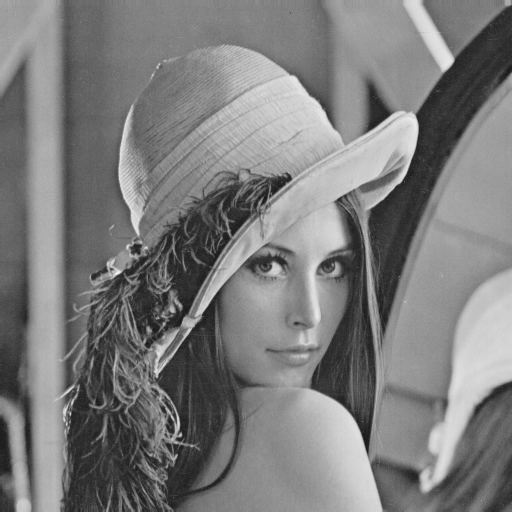
\includegraphics{C:/Users/Jamie/Documents/University-Stuffs/MAT3007/Midterm/test_images/512_512_lena.png}
&
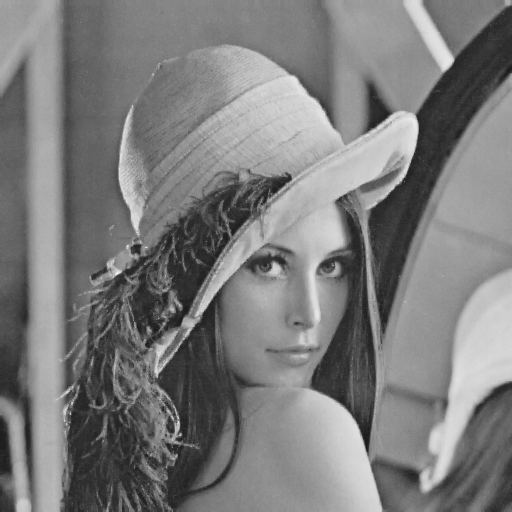
\includegraphics{C:/Users/Jamie/Documents/University-Stuffs/MAT3007/Midterm/test_results/lena-random50-interior-point-34.5214-19.0156.png}
&
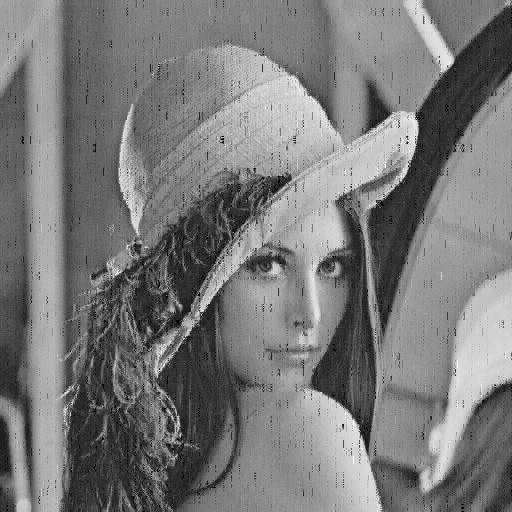
\includegraphics{C:/Users/Jamie/Documents/University-Stuffs/MAT3007/Midterm/test_results/delta_cmp/512_lena+rand_50_del0.006_276s_26.3.png}
&
\includegraphics{C:/Users/Jamie/Documents/University-Stuffs/MAT3007/Midterm/test_results/delta_cmp/512_lena+rand_50_del0.06_186s_22.6.png}
&
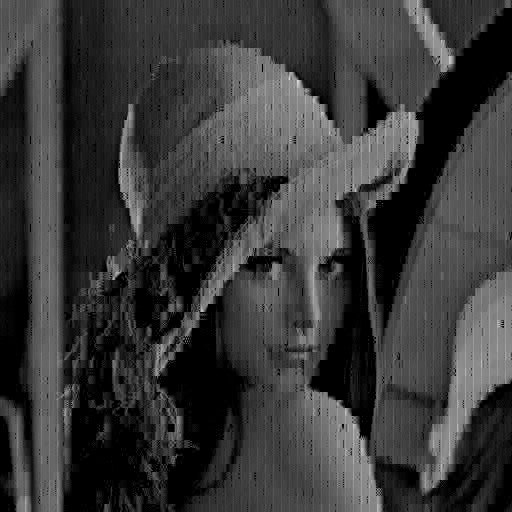
\includegraphics{C:/Users/Jamie/Documents/University-Stuffs/MAT3007/Midterm/test_results/delta_cmp/512_lena+rand_50_del0.3_196s_11.3.png}
&
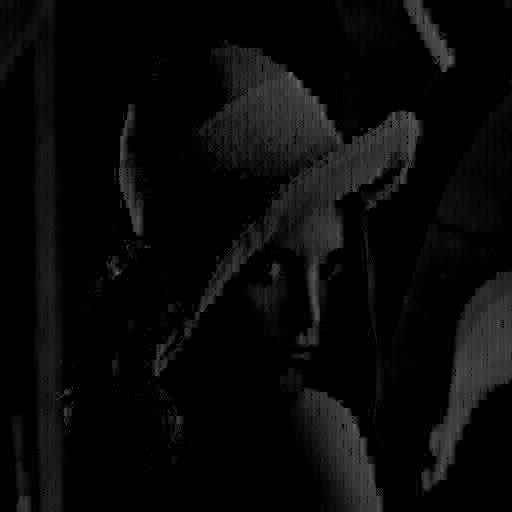
\includegraphics{C:/Users/Jamie/Documents/University-Stuffs/MAT3007/Midterm/test_results/delta_cmp/512_lena+rand_50_del0.6_194s_6.5.png}\tabularnewline
\textbf{PSNR} & - & \(34.5\) & \(26.3\) & \(22.6\) & \(11.3\) &
\(6.5\)\tabularnewline
\textbf{Runtime (Iterations)} & - & \(11.0\text{ sec}\ (11)\) &
\(4.6\text{ min}\ (30)\) & \(3.1\text{ min}\ (21)\) &
\(3.3\text{ min}\ (22)\) & \(3.2\text{ min}\ (21)\)\tabularnewline
\bottomrule
\end{longtable}

\emph{Table 6.} Effects of adjusted \(\delta\) on \(\ell_1\) inpainting
results of \(512\times512\) images contaminated by \(50\%\) random
noise, \(\text{bsz}=8,\) constraint tolerance \(= 10^{-3},\) optimality
tolerance \(= 10^{-6},\) TV model result included for comparison

\hypertarget{header-n249}{%
\subsubsection{Denoising}\label{header-n249}}

We finally test the \(\ell_1\) block model under the denoising setting:
\(A=I_{mn},b=u+\sigma\text{randn}(mn,1)\) where \(A,b,u\) are as in the
TV minimization model, and \(\text{randn}\) adds scaled Gaussian white
noise to the stacked image \(u\). The following results are obtained
with parameters set at \(\sigma=0.1,\delta=0.9\sigma,\text{bsz}=8.\)

\begin{longtable}[]{@{}lll@{}}
\toprule
\textbf{Ground Truth} & GT + Gaussian Noise & Denoised
Image\tabularnewline
\midrule
\endhead
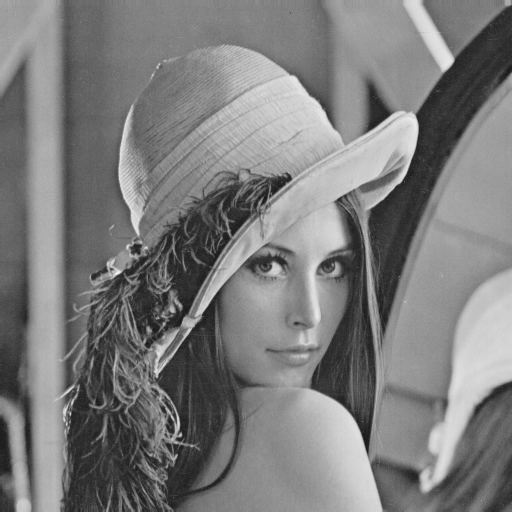
\includegraphics{C:/Users/Jamie/Documents/University-Stuffs/MAT3007/Midterm/test_images/512_512_lena.png}
&
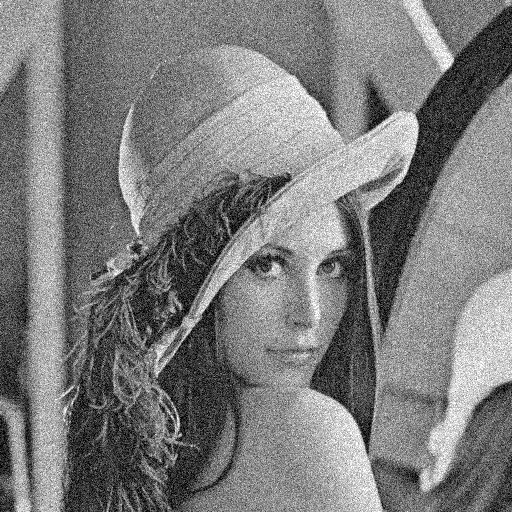
\includegraphics{C:/Users/Jamie/Documents/University-Stuffs/MAT3007/Midterm/test_results/denoise/noised.PNG}
&
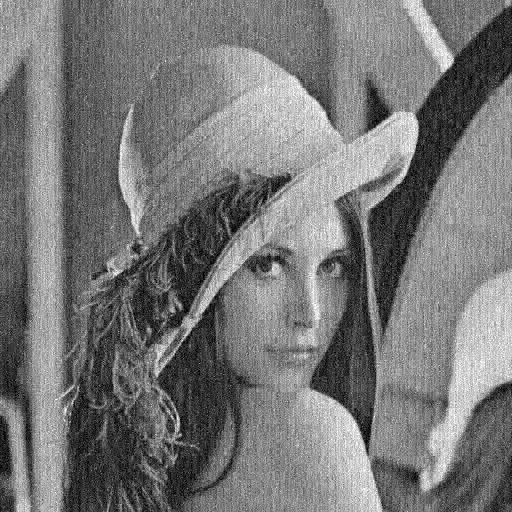
\includegraphics{C:/Users/Jamie/Documents/University-Stuffs/MAT3007/Midterm/test_results/denoise/denoised.PNG}\tabularnewline
\textbf{PSNR} & \(5.7\) & \(22.8\)\tabularnewline
\bottomrule
\end{longtable}

\emph{Table 7.} \(\ell_1\) denoising result of \(512\times512\) images
contaminated by Gaussian white noise,
\(\sigma=0.1,\delta=0.9\sigma,\text{bsz}=8.\)

\hypertarget{header-n266}{%
\subsection{Conclusion}\label{header-n266}}

The overall performance of the \(\ell_1\) image inpainting model were
unsatisfactory in terms of reconstruction quality and running speed. On
all sample images we tested, the \(\text{PSNR}\) of the model's
reconstruction results fell well short of \(30,\) a benchmark easily
obtained by the TV model; the speed of the \(\ell_1\) model was also
significantly slower than the TV model. With \(\text{bsz}=8\) the
typical runtime of reconstructing a \(512\times512\) image was
\(3\text{ min}\) - \(5 \text{ min}\) in \(20\) - \(30\) iterations,
while the TV model could achieve better results in around \(10\)
seconds, \(10\) iterations. The reason for the slow running speed might
be due to a relatively dense \(\Psi\) matrix, which led to a large
amount of computation. Better reconstruction results might be obtained
by choosing larger \(\text{bsz}\) such as \(16\) or \(32,\) however the
density of \(\Psi\) would also grow quadratically to \(\text{bsz},\)
rendering the task almost impossible on a regular PC.

We discovered that the model produced better results when reconstructing
images with evenly-spread damage - which might be explained by the
damage's correspondence to higher frequencies after transformed by
\(\Psi.\) We found that neither the optimality tolerance nor the
constraint tolerance had a significant impact on the quality or runtime
of the reconstruction. Nevertheless, the program might experience
instability and some indefinite behavior with optimality tolerance
\(\gt10^{-4}\) or constraint tolerance \(\lt10^{-6}.\) We also found
that smaller \(\delta\) produced better reconstruction results, while
sacrificing some speed when \(\delta<0.01.\) The program might
experience instability when \(\delta\) was below \(0.006.\) Finally, we
found that the \(\ell_1\) model might be suitable for denoising tasks
(in which the positions of noise signals are unknown).

\end{document}
